% @author Arian Helberg

\chapter{Einleitung}

\gls{ac:haw}~\gls{sy:ohm}~\gls{gl:haw}(Damit das glossar keine fehler schmeißt)

Effizientes Objektdesign und -modellierung sind entscheidende Kernkompetenzen in verschiedenen Bereichen der
digitalen Welt.
Da die Erstellung geometrischer Objekte für Laien unintuitiv ist und ein großes Maß an Erfahrung und Expertise
erfordert, ist dieses stetig wachsende Feld für Neueinsteiger nur sehr schwer zu erschließen.
Die Forschung liefert hierzu einige Arbeiten zur prozeduralen Modellierung, um digitale Inhalte schneller
und automatisiert zu erstellen.
Gerade wenn es um die Darstellung natürlicher Umgebung geht, ist die Erstellung von ähnlichen Objekten, wie
zum Beispiel verschiedene Bäume derselben Gattung eines Waldes, ein schwieriges Problem.
Kleine Änderungen in prozeduralen Systemen können zu großen Veränderungen der Ergebnisse führen.
Darum beschäftigt sich die inverse prozedurale Modellierung unter anderem mit dem Inferieren von Regeln
und Mustern aus gegeben Objekten, um diese nach bestimmten Regeln zu modellieren.
Ein wichtiges Werkzeug hierbei ist die Verwendung formaler Grammatiken als fundamentale Datenstruktur
der Informatik, um Strukturen zu beschreiben.
Eine spezielle Untergruppe sind die L-Systeme, die häufig bei der Beschreibung
von Verzweigungsstrukturen und Selbstähnlichkeit zum Einsatz kommen.
\\~\\
Diese Arbeit soll sich mit der Erstellung eines prozeduralen Systems zur Synthese von Ähnlichkeitsabbildern
beschäftigen.
Hierzu soll über eine Benutzerschnittstelle eine Struktur erzeugt werden, aus der ein parametrisiertes L-Systems
inferiert werden kann, das dann zur Generierung von ähnlichen Strukturen genutzt werden kann.

\newpage

\section{Problemstellung}

Mit der Digitalisierung der Welt steigt auch der Bedarf an digitalen Inhalten.
Zu den größten Feldern gehören Gaming- und Unterhaltungsindustrie, Datenvisualisierung und interaktive Anwendungen.
Um eine erhöhte Quantität dieser Inhalte liefern zu können, werden Methodiken und Algorithmen gesucht, die eine Erstellung
vereinfachen.
Während Methodiken zur Kodifizierung bestimmter Strukturen in den Bereich der prozeduralen Modellierung fällt,
findet das Ableiten von Regeln Anwendung in der inversen prozeduralen Modellierung.
Weiter steigt mit dem digitalen und naturwissenschaftlichen Fortschritt die Anwendung immer komplexerer Strukturen, die
ein Herausarbeiten der schwer zu kontrollierenden, prozeduralen Regeln immer schwieriger machen.
\\~\\
Ein Beispiel hierzu aus der Gaming-Industrie ist die frühere Verwendung unorganisierter Modelle.
Unorganisierte Modelle sind nur bedingt Wiederverwendtbar, da nur die vorliegende Modellierung verwendet werden kann.
Es besteht eine hohe Speicherkomplexität bei geringer Laufzeitkomplexität.
Für kleinste Veränderungen am Modell ist eine erneute Modellierung nötig, die wiederum Speicher benötigt, um sie
persistent speichern zu können.
Heutzutage werden die Objekte nach bestimmten Kriterien organisiert, um eine austomatisierte Modellierung durch Algorithmen
zu ermöglichen, um so aus einer Grundstruktur weitere Modelle zu erzeugen.
Speicher- und Laufzeitkomplexität nähern sich an.
Deshalb werden allgemeingültige, vielseitig anwendbare Algorithmen gesucht, die bestimmte natürliche Eigenschaften
von Strukturen herausarbeiten ("`Reverse Engineering"'), um diese für die (inverse) prozedurale Modellierung zur
Verfügung zu stellen.
\\~\\
Diese Arbeit soll zeigen, wie sich durch die Erstellen eines Systems zur Generierung von ähnlichen Strukture aus einer
Basistruktur aktuelle Ansätze aus der Forschung in einem Programm umsetzen lassen.

\newpage

\section{Ziele}

Die Erstellung eines Systems zur Synthese von ähnlichen Struktures aus einer Basisstruktur soll zentrale Aufgabe dieser
Arbeit sein.
Aus der Fragestellung leiten sich folgende Teilziele ab:

\begin{itemize}
    \item Die Erstellung eines Programms zur Umsetzung des erstellten Systems
    \item Anwenden von Algorithmen und Ansätzen der aktuellen Forschung
    \item Testen von Metriken und deren Auswirkung auf das Ergebnis
    \item Erstellung eigener Methodiken und Algorithmen zur Effizienten Lösung der Problemstellung
    \item Schaffen eines Teilsystems zum Extrahieren von Eigenschaften und Regeln einer Basisstruktur
\end{itemize}

Die Erstellung und Integration eines neuronalen Netzes, das laut aktueller Forschung gute Ergebnisse beim Lernen von
Regeln aus einer Eingabestruktur liefert, kann in dieser Arbeiten aus Praktikabilitätsgründen nicht behandelt werden.

\section{Methodik}

\textit{Abbildung 1 zeigt, wie das o.g. System aufgebaut ist}:
\begin{itemize}
    \item[I.] \underline{Strukturieren}: Der Benutzer nutzt die grafische Benutzerschnittstelle, um aus
    einzelnen, atomaren Strukturen (\textbf{Templates}) eine zusammenhängende Struktur zu erstellen.
    Neben der Position der Templates können auch Parameter wie Rotation angepasst
    werden.
    \item[II.] \underline{Visualisieren}: Das Ergebnis der Strukturierung ist jederzeit sichtbar.
    Einfache Liniensegmente können mit einem \textbf{Turtle-Algorithmus} gezeichnet werden.
    \item[III.] \underline{Datengenerierung}: Das Ergebnis der Strukturierung wird in einer Baumstruktur
    organisiert, in der jeder Knoten einem bestimmten Template entspricht und die zugehörigen Kanten die
    geometrischen Transformationen relativ zum Elternknoten beschreibt.
    \item[IV.] \underline{Inferieren}: Aus der Baumstruktur kann eine formale Grammatik in Form eines kleinen
    L-Systems abgeleitet werden, indem identische topologische Strukturen (Unterbäume) gefunden werden können.
    \item[V.] \underline{Optimieren}: Hier werden ähnliche Produktionsregeln des L-Systems mithilfe einer
    \textbf{Kostenfunktion}\footnote[1]{Die Kostenfunktion setzt sich sowohl aus der Länge der Grammatik, als
    auch der Distanz von der alten zur neuen, generalisierten Grammatik nach dem Merge zusammen} zusammengefasst
    (\textit{engl. Merge}), um diese mit nicht-deterministischen Regeln und Rekursion zu generalisieren.
    \item[VI.] \underline{Randomisieren}: Jedes Symbol der Grammatik nimmt eine Liste an Parametern entgegen, die
    in diesem Schritt nach bestimmten Kriterien pseudo-randomisiert werden, um Variationen zu erstellen und
    anschließend zu visualisieren.
\end{itemize}

\section{Aufbau}

Im Folgenden wird auf die Methodik zum Ableiten eines L-Systems eingegangen und Konzepte und eigene Lösungsansätze
präsentiert.

\begin{figure}[H]
    \centering
    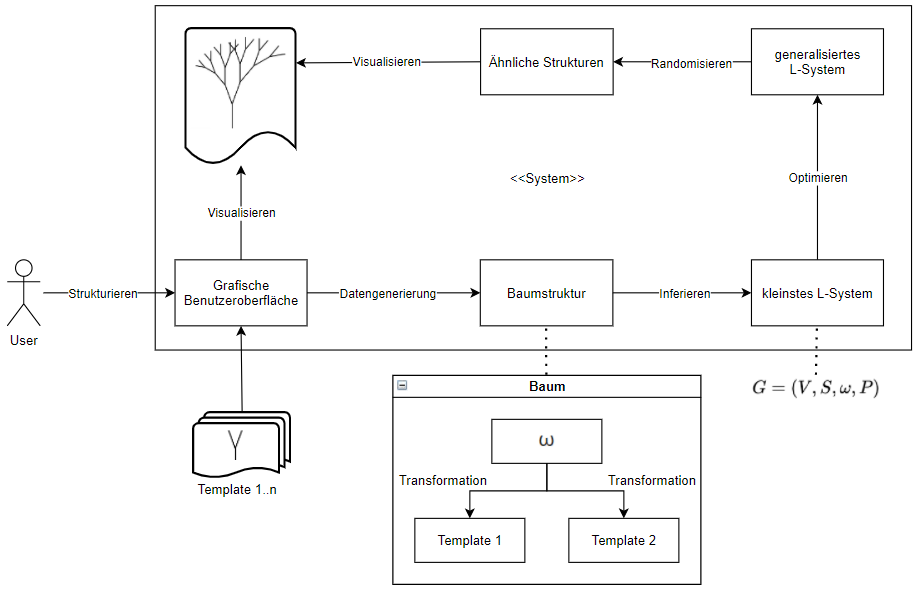
\includegraphics[width=14cm]{../images/System.PNG}
    \caption[Systemarchitektur]{Architektur des Systems mit einigen Datenstrukturen}
\end{figure}

\subsubsection{System}
Ziel des Systems ist die Erstellung von Ähnlichkeitsabbildern einer Struktur, die über eine grafische
Benutzeroberfläche erstellt wird.